\chapter{Detalhes da Implementação}

\section{Introdução}

Este capítulo descreve os detalhes da implementação do sistema de treinamento e inserção automática desenvolvida para gerar ambientes virtuais a partir de imagens. A aplicação foi desenvolvida para automatizar tanto o treinamento do modelo de reconhecimento de objetos quanto a geração de modelos tridimensionais a partir das imagens processadas.

O principal objetivo da implementação é oferecer ao usuário uma experiência simplificada de criação de ambientes virtuais, a partir do carregamento de imagens em um menu intuitivo dentro da plataforma Unity. Essa abordagem reduz a necessidade de intervenção manual, tornando o processo mais eficiente e acessível para usuários que desejam criar ambientes 3D rapidamente.

\subsection{Estrutura geral da aplicação}

A estrutura da aplicação desenvolvida neste trabalho está esquematizada na Figura \ref{fig:estrutura}. A arquitetura compreende quatro elementos principais que trabalham em conjunto para realizar a tarefa de criação de ambientes virtuais. O processo começa com o treinamento do modelo YOLO que gera os pesos da RNC usados para o reconhecimento dos objetos nas imagens fornecidas.

\begin{figure}[!h]
    \centering
    \begin{minipage}{1\linewidth}
    \centering
    \captionsetup{justification=centering,margin=0.5cm,font=small}
    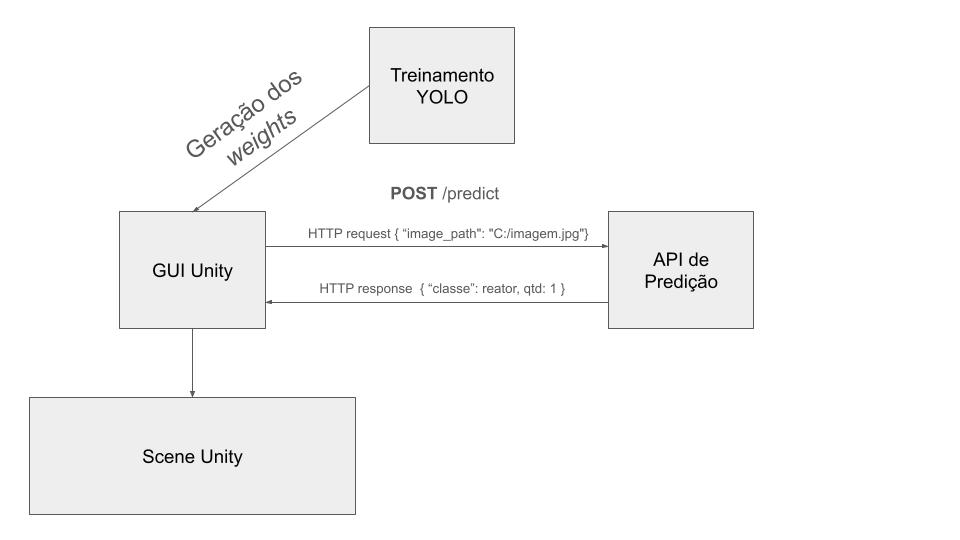
\includegraphics[width=1\linewidth]{img/cap5/estrutura.jpg}
    \caption{Estrutura geral da Aplicação}.
    \label{fig:estrutura}
    \end{minipage}
\end{figure}

O próximo elemento destacado na estrutura é a interface gráfica do usuário (\textit{Graphical User Interface} - GUI) no Unity, ilustrada na Figura \ref{fig:GUI}. Essa interface foi projetada para facilitar a identificação e modelagem da cena. O script desenvolvido para a GUI integra-se diretamente ao Unity, fornecendo uma ferramenta que permite ao usuário selecionar uma imagem e realizar o processamento de reconhecimento. A GUI envia uma requisição HTTP para uma API que aplica o modelo de reconhecimento treinado à imagem fornecida.

Conforme mostrado no diagrama, a API recebe o caminho da imagem, aplica os pesos treinados da RNC e retorna ao Unity a quantidade de objetos identificados e suas respectivas classes. Como o sistema ainda não implementa a localização espacial dos objetos, os modelos virtuais gerados são dispostos uniformemente na cena do Unity após o processamento da imagem.

\begin{figure}[!h]
    \centering
    \begin{minipage}{0.49\linewidth}
        \centering
        \captionsetup{justification=centering,margin=0.5cm,font=small}
        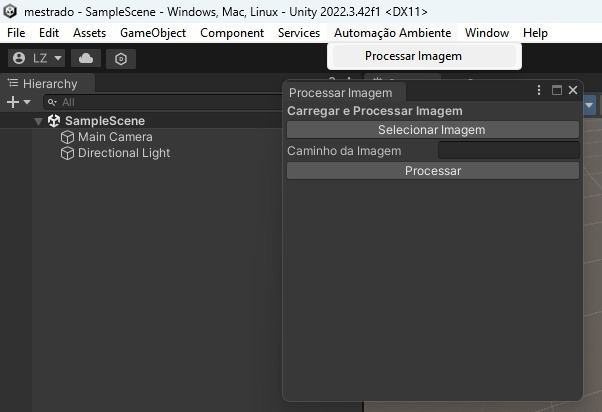
\includegraphics[width=\linewidth]{img/cap5/GUI-TOOL.jpeg}
        \caption{Interface para o usuário.}
        \label{fig:GUI}
    \end{minipage}
\end{figure}

\subsection{Treinamento com a YOLO}

O treinamento com a YOLO segue um padrão comum entre suas diferentes versões, embora cada versão possa exigir pacotes específicos e diferentes processos de instalação. No caso do YOLOv8, o treinamento envolve a importação dos pacotes necessários, a seleção da arquitetura da rede neural (como 'yolov8n.pt') e a execução do treinamento com parâmetros ajustáveis, como o número de épocas e o tipo de otimizador.

A estrutura básica do script de treinamento da YOLOv8 se constitui na importação dos pacotes necessários para funcionamento do modelo, presentes geralmente nas primeiras linhas do arquivo, seguido pela escolha da arquitetura de treinamento, no caso ‘yolov8n.pt’, seguido, por fim, da linha responsável pela execução do treinamento, recebendo como parâmetros as características da rede neural, como a quantidade de épocas, o tipo do otimizador, dentre diversos outros (Figura \ref{fig:script-yolov8}).

\begin{figure}[!h]
    \centering
    \begin{minipage}{0.6\linewidth}
    \centering
    \captionsetup{justification=centering,margin=0.5cm,font=small}
    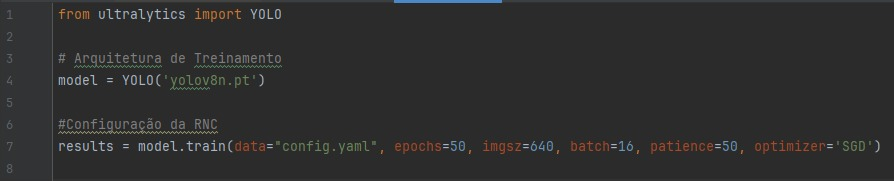
\includegraphics[width=1\linewidth]{img/cap5/treinamentoYOLOv8.jpeg}
    \caption{Demonstração do Script de Treinamento da YOLOv8}.
    \label{fig:script-yolov8}
    \end{minipage}
\end{figure}

\subsection{API de Identificação}

A construção da aplicação responsável pelo processamento das imagens enviadas pelo Unity, resumiu-se à criação de um \textit{endpoint}, ou seja, de uma possibilidade de solicitação do serviço de processamento para aplicações externas. Para acessá-lo, o Unity, deve solicitar o endereço "localhost:5000/predict", com as informação do caminho da imagem dentro do corpo da requisição. Isso fará que seja acessado o método que irá aplicar a função específica da predição, existente dentro dos pacotes da YOLO. Por fim, é percorrido o resultado da predição e extraído dela apenas as informações de interesse para a resposta da requisição, no caso, a quantidade de reatores identificados.    

\begin{figure}[!h]
    \centering
    \begin{minipage}{0.7\linewidth}
    \centering
    \captionsetup{justification=centering,margin=0.5cm,font=small}
    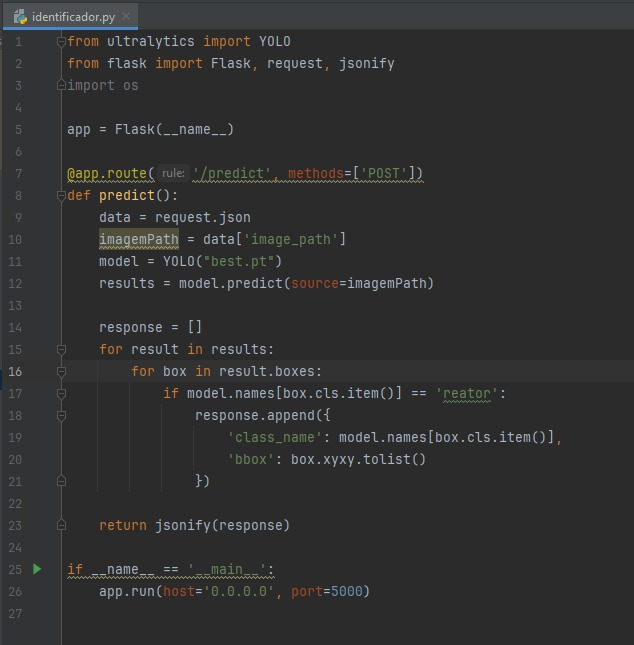
\includegraphics[width=1\linewidth]{img/cap5/API.jpeg}
    \caption{\textit{API} de identificação de imagem}.
    \label{fig:script-yolov8}
    \end{minipage}
\end{figure}


\subsection{Implementação no Unity}

O script desenvolvido no Unity é dividido em alguns métodos. Inicialmente, há a disposição na tela da interface gráfica, representada na Figura \ref{fig:metodo-gui}. Nesse trecho de código, lê-se que é definido o nome da janela desenvolvida, assim como suas dimenções e o tipo de interação que existirá entre o usuário, como selecionar um aimagem, realizar o processamento.

\begin{figure}[!h]
    \centering
    \begin{minipage}{0.7\linewidth}
    \centering
    \captionsetup{justification=centering,margin=0.5cm,font=small}
    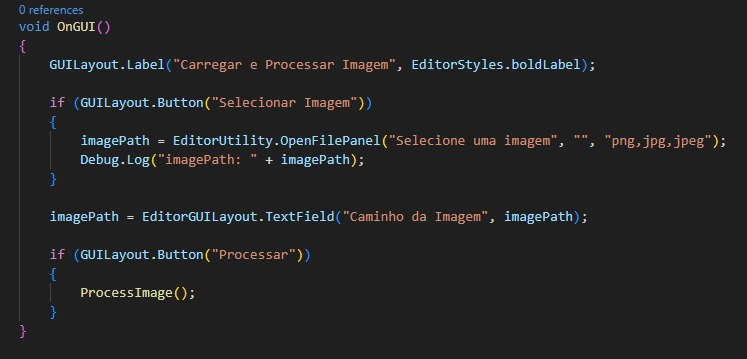
\includegraphics[width=1\linewidth]{img/cap5/gui-codigo.jpeg}
    \caption{\textit{API} de identificação de imagem}.
    \label{fig:metodo-gui}
    \end{minipage}
\end{figure}

Ao precionar o botão de processamento construído no método anterior, é realizada a ação da Figura \ref{fig:metodo-disposicao}. Neste método, é invocado outro método para realização da requisição do processamento, assim como o envio do caminho da imagem e o tratamento da resposta recebida. Com essas informações, realiza-se um iteração sobre cada objeto identificado, e para cada um, é feita um inserção na cena do Unity.

\begin{figure}[!h]
    \centering
    \begin{minipage}{0.7\linewidth}
    \centering
    \captionsetup{justification=centering,margin=0.5cm,font=small}
    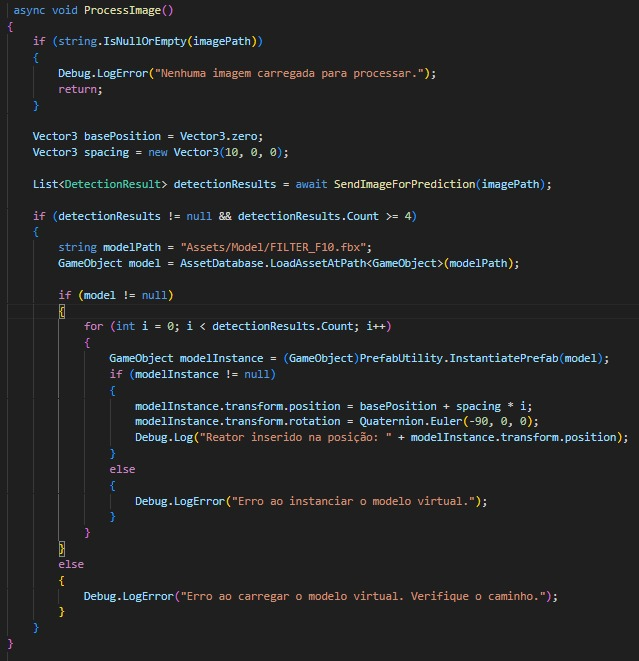
\includegraphics[width=1\linewidth]{img/cap5/process-image.jpeg}
    \caption{Método de processamento da imagem e inserção dos modelos conforme a resposta da API}.
    \label{fig:metodo-disposicao}
    \end{minipage}
\end{figure}


Ao precionar o botão de processamento construído no método anterior, é \textit{renderizado}, ou seja, inserido na tela do Unity o número de reatores identificados na foto. Na Figura \ref{fig:predict}, visualiza-se a imagem processada e seu resultado, que no caso foram de quatro reatores. A quantidade de reatores inseridos naturalmente dependerá da acurácia do modelo assim como a quantidade de elemtnos identificáveis na foto.


\begin{figure}[!h]
    \centering
    \begin{minipage}{0.7\linewidth}
    \centering
    \captionsetup{justification=centering,margin=0.5cm,font=small}
    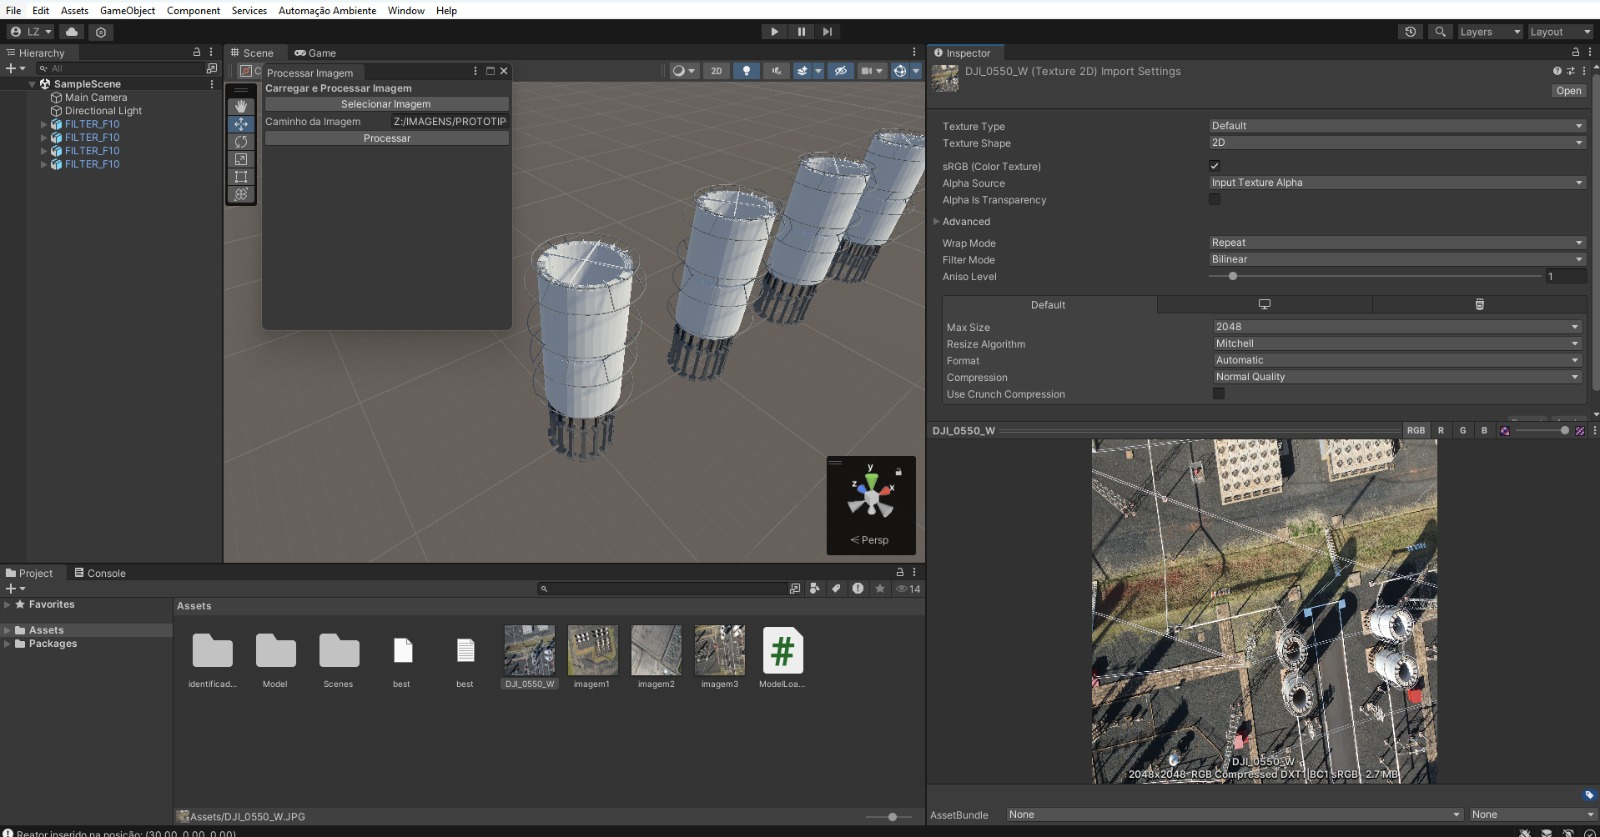
\includegraphics[width=1\linewidth]{img/cap5/predict.jpeg}
    \caption{Método de processamento da imagem e inserção dos modelos conforme a resposta da API}.
    \label{fig:predict}
    \end{minipage}
\end{figure}

\subsection{Conclusão}

A implementação é de uso intuitivo e facilitado. Para executá-la em um computador pessoa, é necessário apenas a inserção do script da direcionado para a Unity dentro do projeto, e em um arquivo separado, executar o código da \textit{API}. No geral, é uma aplicação que se apresenta como uma solução simplificada e com importante impacto no desenvolvimento de ambientes de realide virutal.


	
